\documentclass[11pt,a4paper]{article}

% Packages
\usepackage[margin=1in]{geometry}
\usepackage{graphicx}
\usepackage{booktabs}
\usepackage{amsmath}
\usepackage{tikz}
\usetikzlibrary{shapes.geometric, arrows.meta, positioning, fit, backgrounds, calc}
\usepackage{xcolor}
\usepackage{enumitem}
\usepackage{caption}
\usepackage{subcaption}
\usepackage{float}
\usepackage{adjustbox}

% Colors
\definecolor{stagezero}{HTML}{E8F5E9}
\definecolor{stageone}{HTML}{E3F2FD}
\definecolor{stagetwo}{HTML}{FFF3E0}
\definecolor{stagethree}{HTML}{F3E5F5}
\definecolor{sheriffcolor}{HTML}{FFEBEE}
\definecolor{autocolor}{HTML}{C8E6C9}
\definecolor{darkgreen}{HTML}{2E7D32}
\definecolor{darkblue}{HTML}{1565C0}
\definecolor{darkorange}{HTML}{E65100}
\definecolor{darkpurple}{HTML}{6A1B9A}
\definecolor{darkred}{HTML}{B71C1C}
\definecolor{graybox}{HTML}{F5F5F5}

\title{\textbf{Cascading Confidence-Gated Triage System}\\[0.5em]
\large System Architecture Overview for Automated\\Performance Alert Classification in Mozilla's Perfherder}
\author{}
\date{}

\begin{document}
\maketitle

% ============================================================
\section{Context: The Performance Regression Problem}
% ============================================================

Modern continuous integration (CI) systems execute thousands of performance tests on every code change. When a test's performance degrades beyond a threshold, the system raises a \textbf{performance alert}---a signal that a code change may have introduced a regression (e.g., slower page load, higher memory usage).

Mozilla's \textbf{Perfherder} system monitors performance across Firefox and related projects. It uses a two-sample Student's T-test with a fixed 2\% threshold to detect regressions in time-series data from approximately 5,655 performance test signatures. This automated detection produces a high volume of alerts: our dataset contains \textbf{17,989 alerts} grouped into \textbf{3,912 alert summaries}.

The critical bottleneck is not detection---it is \textbf{triage}. Currently, human engineers called \textit{sheriffs} manually review every alert to determine whether it represents a real regression, what action to take, and whether a bug report should be filed. This is time-consuming, subjective, and does not scale.

\vspace{0.5em}
\noindent\fbox{\parbox{\dimexpr\linewidth-2\fboxsep-2\fboxrule}{%
\textbf{Goal:} Build a cascading ML system that automates the triage of performance alerts, confidently resolving straightforward cases and routing ambiguous ones to human sheriffs---reducing manual workload by an estimated 48--55\%.
}}

% ============================================================
\section{Key Definitions}
% ============================================================

\begin{description}[leftmargin=1.5cm, style=nextline]

\item[\textsf{Alert}]
A single performance test that exceeded the regression detection threshold. Each alert belongs to one test signature (e.g., ``page-load speed on Linux'') and carries metadata: magnitude of change, T-test statistic, test suite, platform, and noise profile.

\item[\textsf{Alert Summary (Group)}]
A collection of alerts triggered by the \textit{same code push}. One push may cause regressions across multiple tests, producing a group of related alerts. Our dataset contains 3,912 summaries averaging 4.6 alerts each. A summary receives a single group-level status and, optionally, a linked bug report.

\item[\textsf{Summary Status}]
A group-level label assigned by a sheriff indicating the disposition of the entire alert summary. Nine possible values exist:

\vspace{0.3em}
\begin{center}
\small
\begin{tabular}{clcc}
\toprule
\textbf{Code} & \textbf{Label} & \textbf{Implies Real?} & \textbf{Summaries} \\
\midrule
0 & Untriaged & Unknown & 656 \\
1 & Downstream & Yes & 30 \\
2 & Reassigned & Yes & 1,224 \\
3 & Invalid & \textbf{No} & 488 \\
4 & Acknowledged & Yes & 692 \\
5 & Investigating & Uncertain & 565 \\
6 & Wontfix & Yes & 158 \\
7 & Fixed & Yes & 84 \\
8 & Backedout & Yes & 15 \\
\bottomrule
\end{tabular}
\end{center}
\vspace{0.3em}

All statuses except \textit{Invalid} and \textit{Untriaged} indicate that the alert represents a genuine performance regression. The distinction between them is the \textit{disposition}---what action was taken (e.g., fixed, reassigned to another team, deemed not worth fixing).

\item[\textsf{Individual Alert Status}]
A per-alert label capturing each alert's role \textit{within} its group. Five possible values: Untriaged (0), Downstream (1), Reassigned (2), Invalid (3), Acknowledged (4). Note that \textit{Investigating}, \textit{Wontfix}, \textit{Fixed}, and \textit{Backedout} exist only at the summary level.

\item[\textsf{has\_bug}]
A binary group-level property indicating whether a bug report was linked to the alert summary (\texttt{alert\_summary\_bug\_number} is not null). Overall rate: 16.2\% of summaries. Strongly correlated with summary status: Backedout $\rightarrow$ 100\%, Acknowledged $\rightarrow$ 37\%, Invalid $\rightarrow$ 0.4\%.

\item[\textsf{Investigating (Model Output)}]
In our system, ``Investigating'' has a different meaning than in the training data. When the \textit{sheriff} marks a group as Investigating, it means they are still reviewing it (a temporary state). When our \textit{model} outputs Investigating, it means the model's confidence is below the decision threshold---it is deferring to a human. This distinction is critical: the model never trains on Investigating labels. They emerge from the confidence gate.

\end{description}

% ============================================================
\section{System Architecture}
% ============================================================

The system operates as a \textbf{cascading pipeline} with four stages. Each stage makes predictions gated by a \textbf{confidence threshold}: only predictions above the threshold are auto-labeled; uncertain cases are deferred to human review. This is known as \textit{selective prediction} or \textit{learning to defer}.

\vspace{1em}

% --- MAIN ARCHITECTURE DIAGRAM ---
\begin{figure}[H]
\centering
\adjustbox{max width=\textwidth}{%
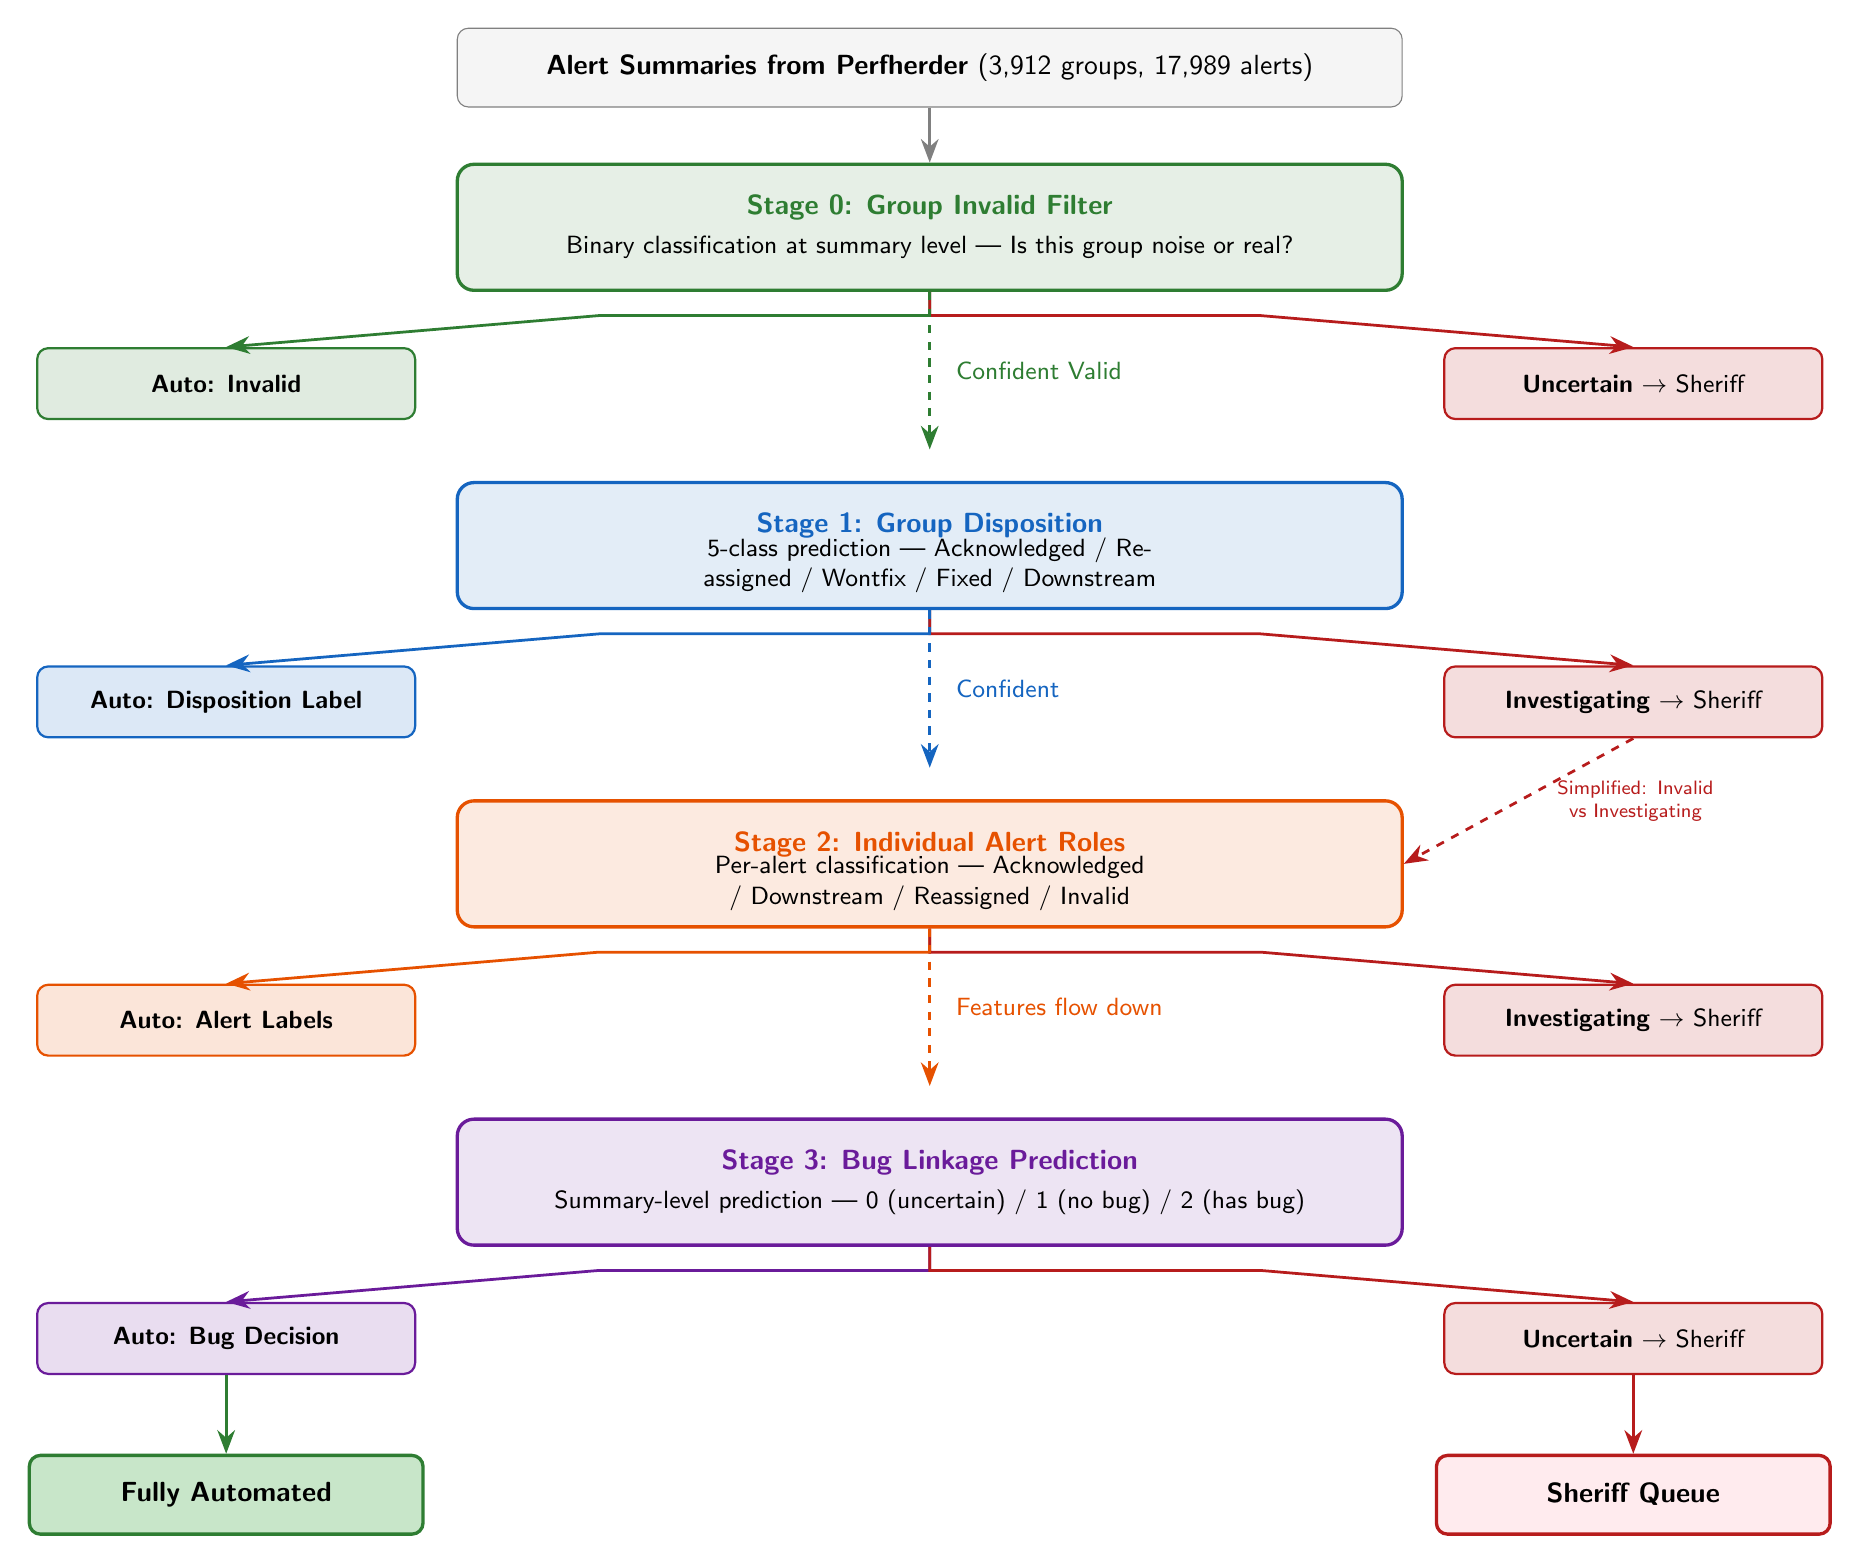
\begin{tikzpicture}[
    node distance=0.6cm and 1.2cm,
    stage/.style={rectangle, rounded corners=6pt, draw=#1, fill=#1!12,
                  line width=1.2pt, minimum width=12cm, minimum height=1.6cm,
                  font=\sffamily},
    output/.style={rectangle, rounded corners=4pt, draw=#1, fill=#1!15,
                   line width=0.8pt, minimum width=4.8cm, minimum height=0.9cm,
                   font=\sffamily\small},
    arrow/.style={-{Stealth[length=3mm]}, line width=1pt, color=#1},
    label/.style={font=\sffamily\footnotesize\color{#1}},
]

% Input
\node[rectangle, rounded corners=4pt, draw=gray, fill=graybox,
      minimum width=12cm, minimum height=1cm, font=\sffamily]
      (input) {\textbf{Alert Summaries from Perfherder} (3,912 groups, 17,989 alerts)};

% Stage 0
\node[stage=darkgreen, below=0.7cm of input] (s0) {};
\node[font=\sffamily\bfseries\color{darkgreen}] at ([yshift=0.25cm]s0.center)
      {Stage 0: Group Invalid Filter};
\node[font=\sffamily\small, text width=10cm, align=center] at ([yshift=-0.25cm]s0.center)
      {Binary classification at summary level --- Is this group noise or real?};

% Stage 0 outputs
\node[output=darkgreen, below left=0.7cm and 0.5cm of s0] (s0_auto)
      {\textbf{Auto: Invalid}};
\node[output=darkred, below right=0.7cm and 0.5cm of s0] (s0_uncertain)
      {\textbf{Uncertain} $\rightarrow$ Sheriff};

% Arrow down center
\node[below=0.7cm of s0] (s0_mid) {};
\draw[arrow=darkgreen] (s0.south) -- ++(0,-0.3cm) -- ++(-4.2cm,0) -- (s0_auto.north);
\draw[arrow=darkred] (s0.south) -- ++(0,-0.3cm) -- ++(4.2cm,0) -- (s0_uncertain.north);

% Valid arrow down
\node[font=\sffamily\small\color{darkgreen}, below=1.7cm of s0] (valid_label) {};
\draw[arrow=darkgreen, dashed] (s0.south) -- ++(0,-2.0cm)
      node[midway, right=0.2cm, font=\sffamily\small\color{darkgreen}] {Confident Valid};

% Stage 1
\node[stage=darkblue, below=2.4cm of s0] (s1) {};
\node[font=\sffamily\bfseries\color{darkblue}] at ([yshift=0.25cm]s1.center)
      {Stage 1: Group Disposition};
\node[font=\sffamily\small, text width=10cm, align=center] at ([yshift=-0.25cm]s1.center)
      {5-class prediction --- Acknowledged / Reassigned / Wontfix / Fixed / Downstream};

% Stage 1 outputs
\node[output=darkblue, below left=0.7cm and 0.5cm of s1] (s1_auto)
      {\textbf{Auto: Disposition Label}};
\node[output=darkred, below right=0.7cm and 0.5cm of s1] (s1_uncertain)
      {\textbf{Investigating} $\rightarrow$ Sheriff};

\draw[arrow=darkblue] (s1.south) -- ++(0,-0.3cm) -- ++(-4.2cm,0) -- (s1_auto.north);
\draw[arrow=darkred] (s1.south) -- ++(0,-0.3cm) -- ++(4.2cm,0) -- (s1_uncertain.north);

% Stage 2
\node[stage=darkorange, below=2.4cm of s1] (s2) {};
\node[font=\sffamily\bfseries\color{darkorange}] at ([yshift=0.25cm]s2.center)
      {Stage 2: Individual Alert Roles};
\node[font=\sffamily\small, text width=10cm, align=center] at ([yshift=-0.25cm]s2.center)
      {Per-alert classification --- Acknowledged / Downstream / Reassigned / Invalid};

\draw[arrow=darkblue, dashed] (s1.south) -- ++(0,-2.0cm)
      node[midway, right=0.2cm, font=\sffamily\small\color{darkblue}] {Confident};
% Also uncertain groups get simplified Stage 2b
\draw[arrow=darkred, dashed, bend right=20] (s1_uncertain.south) -- (s2.east)
      node[midway, right=0.1cm, font=\sffamily\scriptsize\color{darkred}, text width=2.5cm, align=center]
      {Simplified: Invalid vs Investigating};

% Stage 2 outputs
\node[output=darkorange, below left=0.7cm and 0.5cm of s2] (s2_auto)
      {\textbf{Auto: Alert Labels}};
\node[output=darkred, below right=0.7cm and 0.5cm of s2] (s2_uncertain)
      {\textbf{Investigating} $\rightarrow$ Sheriff};

\draw[arrow=darkorange] (s2.south) -- ++(0,-0.3cm) -- ++(-4.2cm,0) -- (s2_auto.north);
\draw[arrow=darkred] (s2.south) -- ++(0,-0.3cm) -- ++(4.2cm,0) -- (s2_uncertain.north);

% Stage 3
\node[stage=darkpurple, below=2.4cm of s2] (s3) {};
\node[font=\sffamily\bfseries\color{darkpurple}] at ([yshift=0.25cm]s3.center)
      {Stage 3: Bug Linkage Prediction};
\node[font=\sffamily\small, text width=10cm, align=center] at ([yshift=-0.25cm]s3.center)
      {Summary-level prediction --- 0 (uncertain) / 1 (no bug) / 2 (has bug)};

\draw[arrow=darkorange, dashed] (s2.south) -- ++(0,-2.0cm)
      node[midway, right=0.2cm, font=\sffamily\small\color{darkorange}] {Features flow down};

% Stage 3 outputs
\node[output=darkpurple, below left=0.7cm and 0.5cm of s3] (s3_auto)
      {\textbf{Auto: Bug Decision}};
\node[output=darkred, below right=0.7cm and 0.5cm of s3] (s3_uncertain)
      {\textbf{Uncertain} $\rightarrow$ Sheriff};

\draw[arrow=darkpurple] (s3.south) -- ++(0,-0.3cm) -- ++(-4.2cm,0) -- (s3_auto.north);
\draw[arrow=darkred] (s3.south) -- ++(0,-0.3cm) -- ++(4.2cm,0) -- (s3_uncertain.north);

% Final outputs
\node[rectangle, rounded corners=4pt, draw=darkgreen, fill=autocolor,
      line width=1.2pt, minimum width=5cm, minimum height=1cm,
      font=\sffamily\bfseries, below=1.0cm of s3_auto] (final_auto)
      {Fully Automated};

\node[rectangle, rounded corners=4pt, draw=darkred, fill=sheriffcolor,
      line width=1.2pt, minimum width=5cm, minimum height=1cm,
      font=\sffamily\bfseries, below=1.0cm of s3_uncertain] (final_sheriff)
      {Sheriff Queue};

\draw[arrow=darkgreen] (s3_auto.south) -- (final_auto.north);
\draw[arrow=darkred] (s3_uncertain.south) -- (final_sheriff.north);

% Top arrow
\draw[arrow=gray] (input.south) -- (s0.north);

\end{tikzpicture}%
}% end adjustbox
\caption{Cascading confidence-gated triage system. Each stage auto-labels confident predictions (left, green path) and defers uncertain cases to human sheriffs (right, red path). Alerts flow downward through stages only when the preceding stage is confident.}
\label{fig:architecture}
\end{figure}

% ============================================================
\section{Stage Descriptions}
% ============================================================

% --- STAGE 0 ---
\subsection{Stage 0: Group Invalid Filter}

\noindent\adjustbox{max width=\textwidth}{%
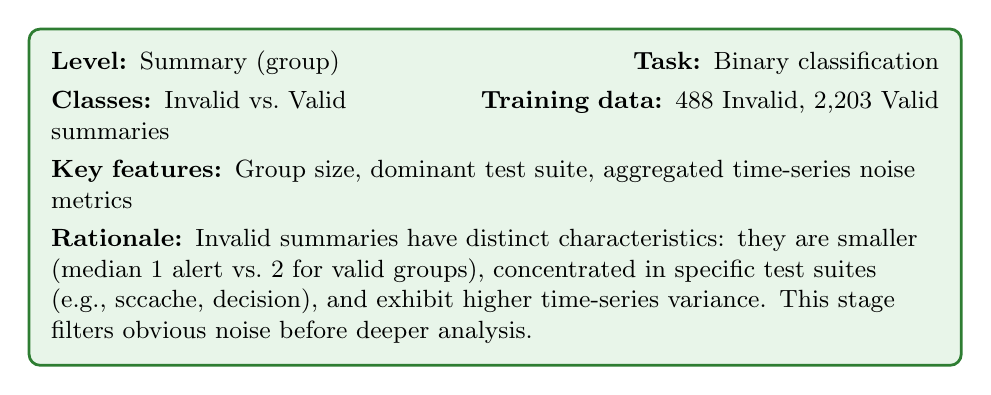
\begin{tikzpicture}
\node[rectangle, rounded corners=4pt, draw=darkgreen, fill=stagezero,
      line width=1pt, text width=0.93\textwidth,
      align=left, font=\small, inner sep=8pt] {
\textbf{Level:} Summary (group) \hfill \textbf{Task:} Binary classification\\[3pt]
\textbf{Classes:} Invalid vs.\ Valid \hfill \textbf{Training data:} 488 Invalid, 2{,}203 Valid summaries\\[3pt]
\textbf{Key features:} Group size, dominant test suite, aggregated time-series noise metrics\\[3pt]
\textbf{Rationale:} Invalid summaries have distinct characteristics: they are smaller (median 1 alert vs.\ 2 for valid groups), concentrated in specific test suites (e.g., sccache, decision), and exhibit higher time-series variance. This stage filters obvious noise before deeper analysis.
};
\end{tikzpicture}%
}

\noindent\textbf{Confidence gate behavior:}
\begin{itemize}[nosep]
    \item \textit{Confident Invalid} $\rightarrow$ auto-label entire group and all alerts as Invalid; set \texttt{has\_bug}~=~1 (no bug).
    \item \textit{Confident Valid} $\rightarrow$ pass group to Stage~1 for disposition prediction.
    \item \textit{Uncertain} $\rightarrow$ assign group status ``Investigating'' and route to sheriff queue.
\end{itemize}

% --- STAGE 1 ---
\subsection{Stage 1: Group Disposition}

\noindent\adjustbox{max width=\textwidth}{%
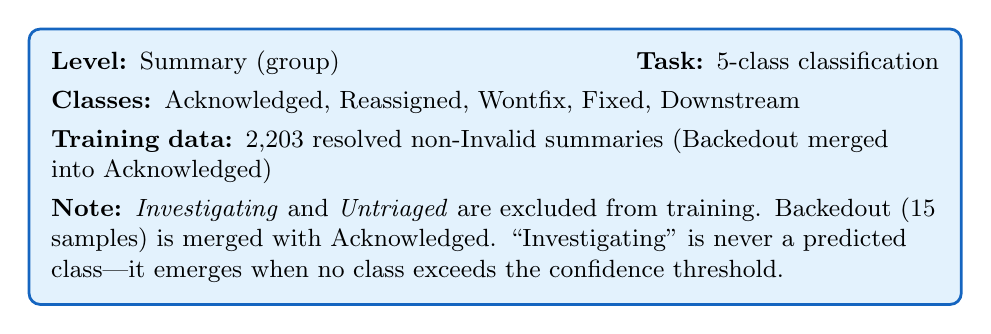
\begin{tikzpicture}
\node[rectangle, rounded corners=4pt, draw=darkblue, fill=stageone,
      line width=1pt, text width=0.93\textwidth,
      align=left, font=\small, inner sep=8pt] {
\textbf{Level:} Summary (group) \hfill \textbf{Task:} 5-class classification\\[3pt]
\textbf{Classes:} Acknowledged, Reassigned, Wontfix, Fixed, Downstream\\[3pt]
\textbf{Training data:} 2{,}203 resolved non-Invalid summaries (Backedout merged into Acknowledged)\\[3pt]
\textbf{Note:} \textit{Investigating} and \textit{Untriaged} are excluded from training. Backedout (15 samples) is merged with Acknowledged. ``Investigating'' is never a predicted class---it emerges when no class exceeds the confidence threshold.
};
\end{tikzpicture}%
}

\noindent\textbf{Confidence gate behavior:}
\begin{itemize}[nosep]
    \item \textit{Confident prediction} $\rightarrow$ auto-label group with the predicted disposition; pass to Stage~2a for individual alert classification.
    \item \textit{Uncertain} $\rightarrow$ assign ``Investigating''; pass to Stage~2b (simplified noise filter only); route group to sheriff queue.
\end{itemize}

\noindent\textbf{Design note:} Many disposition labels (Fixed, Wontfix) reflect post-triage human decisions that are inherently difficult to predict from alert metadata alone. The system compensates by deferring uncertain predictions rather than guessing---only auto-labeling when confident.

% --- STAGE 2 ---
\subsection{Stage 2: Individual Alert Roles}

This stage operates in two modes depending on the outcome of Stage~1:

\vspace{0.5em}
\noindent\textbf{Stage 2a --- Full classification} (for groups with a confident disposition from Stage~1):

\noindent\adjustbox{max width=\textwidth}{%
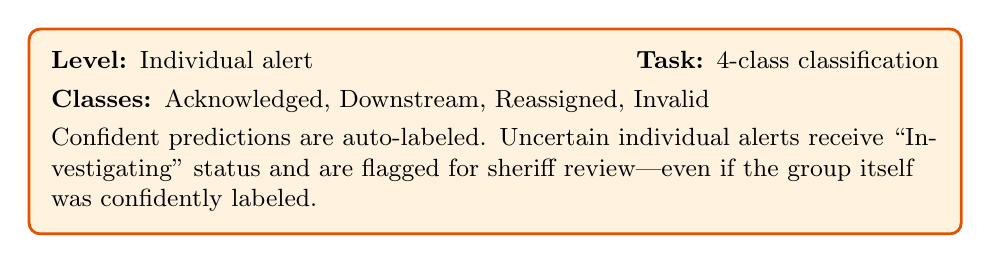
\begin{tikzpicture}
\node[rectangle, rounded corners=4pt, draw=darkorange, fill=stagetwo,
      line width=1pt, text width=0.93\textwidth,
      align=left, font=\small, inner sep=8pt] {
\textbf{Level:} Individual alert \hfill \textbf{Task:} 4-class classification\\[3pt]
\textbf{Classes:} Acknowledged, Downstream, Reassigned, Invalid\\[3pt]
Confident predictions are auto-labeled. Uncertain individual alerts receive ``Investigating'' status and are flagged for sheriff review---even if the group itself was confidently labeled.
};
\end{tikzpicture}%
}

\noindent\textbf{Stage 2b --- Simplified noise filter} (for Investigating groups from Stage~1):

\noindent\adjustbox{max width=\textwidth}{%
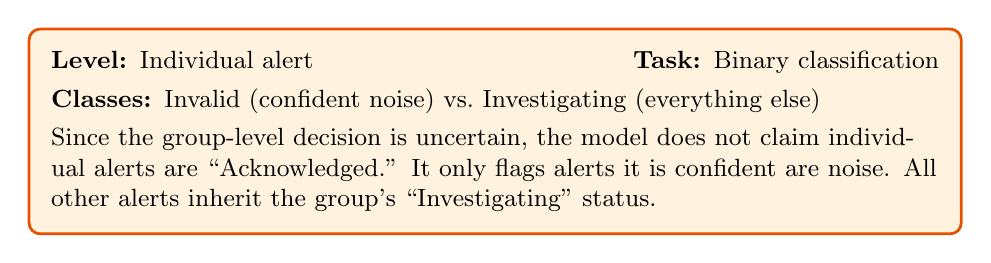
\begin{tikzpicture}
\node[rectangle, rounded corners=4pt, draw=darkorange, fill=stagetwo,
      line width=1pt, text width=0.93\textwidth,
      align=left, font=\small, inner sep=8pt] {
\textbf{Level:} Individual alert \hfill \textbf{Task:} Binary classification\\[3pt]
\textbf{Classes:} Invalid (confident noise) vs.\ Investigating (everything else)\\[3pt]
Since the group-level decision is uncertain, the model does not claim individual alerts are ``Acknowledged.'' It only flags alerts it is confident are noise. All other alerts inherit the group's ``Investigating'' status.
};
\end{tikzpicture}%
}

% --- STAGE 3 ---
\subsection{Stage 3: Bug Linkage Prediction (\texttt{has\_bug})}

\noindent\adjustbox{max width=\textwidth}{%
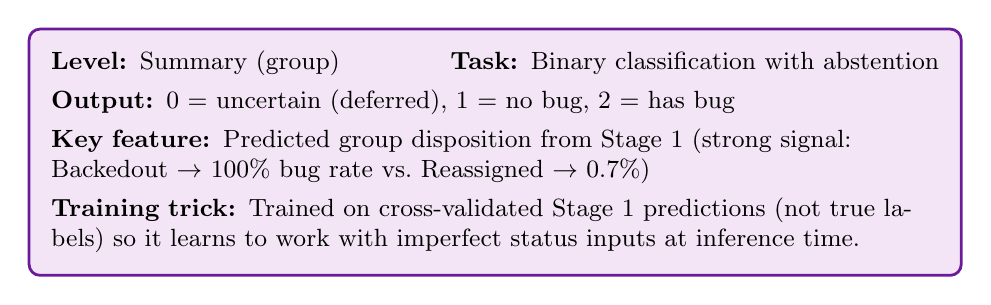
\begin{tikzpicture}
\node[rectangle, rounded corners=4pt, draw=darkpurple, fill=stagethree,
      line width=1pt, text width=0.93\textwidth,
      align=left, font=\small, inner sep=8pt] {
\textbf{Level:} Summary (group) \hfill \textbf{Task:} Binary classification with abstention\\[3pt]
\textbf{Output:} 0 = uncertain (deferred), 1 = no bug, 2 = has bug\\[3pt]
\textbf{Key feature:} Predicted group disposition from Stage~1 (strong signal: Backedout $\rightarrow$ 100\% bug rate vs.\ Reassigned $\rightarrow$ 0.7\%)\\[3pt]
\textbf{Training trick:} Trained on cross-validated Stage~1 predictions (not true labels) so it learns to work with imperfect status inputs at inference time.
};
\end{tikzpicture}%
}

\noindent\textbf{Shortcut rules} (no model needed):
\begin{itemize}[nosep]
    \item Invalid groups (from Stage~0) $\rightarrow$ \texttt{has\_bug}~=~1 (no bug). Only 0.4\% of Invalid groups have bugs.
    \item Reassigned groups (from Stage~1) $\rightarrow$ \texttt{has\_bug}~=~1 (no bug). Only 0.7\% have bugs.
\end{itemize}

\noindent\textbf{Two prediction modes:}
\begin{itemize}[nosep]
    \item \textit{Mode A} (confident group status available): Uses predicted disposition as a feature. Higher expected accuracy.
    \item \textit{Mode B} (Investigating groups): Predicts without status context. The prediction serves as a \textit{hint} for the sheriff, not a final decision.
\end{itemize}

% ============================================================
\section{The Confidence Gate Mechanism}
% ============================================================

The core principle of the system is \textbf{selective prediction}: the model only auto-labels when it is sufficiently confident. This is implemented through calibrated probability thresholds at each stage.

\begin{figure}[H]
\centering
\adjustbox{max width=\textwidth}{%
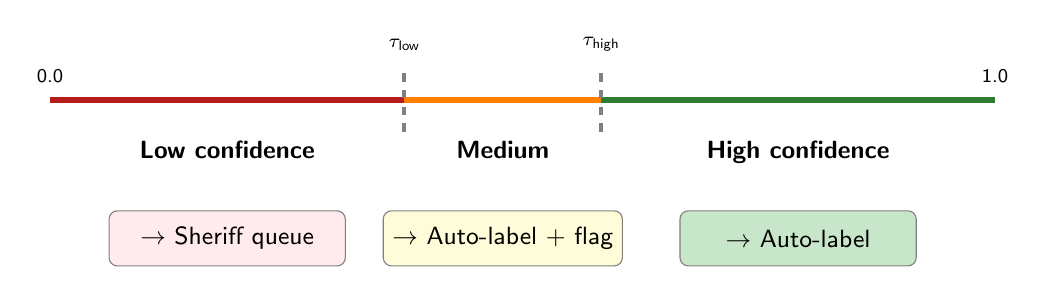
\begin{tikzpicture}[
    node distance=0.4cm,
    box/.style={rectangle, rounded corners=3pt, draw=gray, minimum width=3cm,
                minimum height=0.7cm, font=\sffamily\small},
]
% Confidence spectrum
\draw[line width=2pt, darkred] (0,0) -- (4.5,0);
\draw[line width=2pt, orange] (4.5,0) -- (7,0);
\draw[line width=2pt, darkgreen] (7,0) -- (12,0);

% Threshold markers
\draw[line width=1.5pt, dashed, gray] (4.5,-0.4) -- (4.5,0.4);
\draw[line width=1.5pt, dashed, gray] (7,-0.4) -- (7,0.4);

% Labels
\node[font=\sffamily\small, below] at (2.25,-0.4) {\textbf{Low confidence}};
\node[font=\sffamily\small, below] at (5.75,-0.4) {\textbf{Medium}};
\node[font=\sffamily\small, below] at (9.5,-0.4) {\textbf{High confidence}};

% Actions
\node[box, fill=sheriffcolor, below=1cm] at (2.25,-0.4) {$\rightarrow$ Sheriff queue};
\node[box, fill=yellow!15, below=1cm] at (5.75,-0.4) {$\rightarrow$ Auto-label + flag};
\node[box, fill=autocolor, below=1cm] at (9.5,-0.4) {$\rightarrow$ Auto-label};

% Threshold labels
\node[font=\sffamily\scriptsize, above] at (4.5, 0.5) {$\tau_{\text{low}}$};
\node[font=\sffamily\scriptsize, above] at (7, 0.5) {$\tau_{\text{high}}$};

% Scale
\node[font=\sffamily\scriptsize] at (0, 0.3) {0.0};
\node[font=\sffamily\scriptsize] at (12, 0.3) {1.0};

\end{tikzpicture}%
}% end adjustbox
\caption{Confidence gate spectrum. Each stage uses calibrated probabilities (via Platt scaling or isotonic regression) to decide whether to auto-label, flag, or defer a prediction. Thresholds are tuned per-stage to balance automation rate against error rate.}
\label{fig:confidence}
\end{figure}

\noindent The label ``Investigating'' is \textbf{never a trained class}. It is the system's way of saying: ``I do not have enough confidence to make this decision---a human should review it.'' This avoids a semantic mismatch with the training data, where ``Investigating'' means the sheriff is still reviewing (a temporary, in-progress state), rather than a final deferral.

% ============================================================
\section{Label Scheme}
% ============================================================

The system uses a unified labeling convention across all outputs:

\begin{center}
\begin{tabular}{cll}
\toprule
\textbf{Code} & \textbf{Meaning} & \textbf{When Assigned} \\
\midrule
\multicolumn{3}{l}{\textit{Summary Status}} \\
0 & Not evaluated / Investigating & Model deferred to sheriff \\
1 & Downstream & Confident prediction (Stage 1) \\
2 & Reassigned & Confident prediction (Stage 1) \\
3 & Invalid & Confident prediction (Stage 0) \\
4 & Acknowledged & Confident prediction (Stage 1) \\
6 & Wontfix & Confident prediction (Stage 1) \\
7 & Fixed & Confident prediction (Stage 1) \\
\midrule
\multicolumn{3}{l}{\textit{Individual Alert Status}} \\
0 & Investigating (uncertain) & Model deferred to sheriff \\
1 & Downstream & Confident prediction (Stage 2a) \\
2 & Reassigned & Confident prediction (Stage 2a) \\
3 & Invalid & Confident prediction (Stage 2a/2b) \\
4 & Acknowledged & Confident prediction (Stage 2a) \\
\midrule
\multicolumn{3}{l}{\textit{Bug Linkage (\texttt{has\_bug})}} \\
0 & Uncertain (not evaluated) & Model deferred to sheriff \\
1 & No bug & Confident prediction or shortcut rule \\
2 & Has bug & Confident prediction \\
\bottomrule
\end{tabular}
\end{center}

\noindent In all three outputs, \textbf{code 0 uniformly means ``not evaluated / uncertain.''} This provides a consistent interface: any downstream consumer of the system's output knows that a 0 requires human attention.

% ============================================================
\section{Training Data Strategy}
% ============================================================

A key design decision is the exclusion of ambiguous labels from training:

\begin{figure}[H]
\centering
\adjustbox{max width=\textwidth}{%
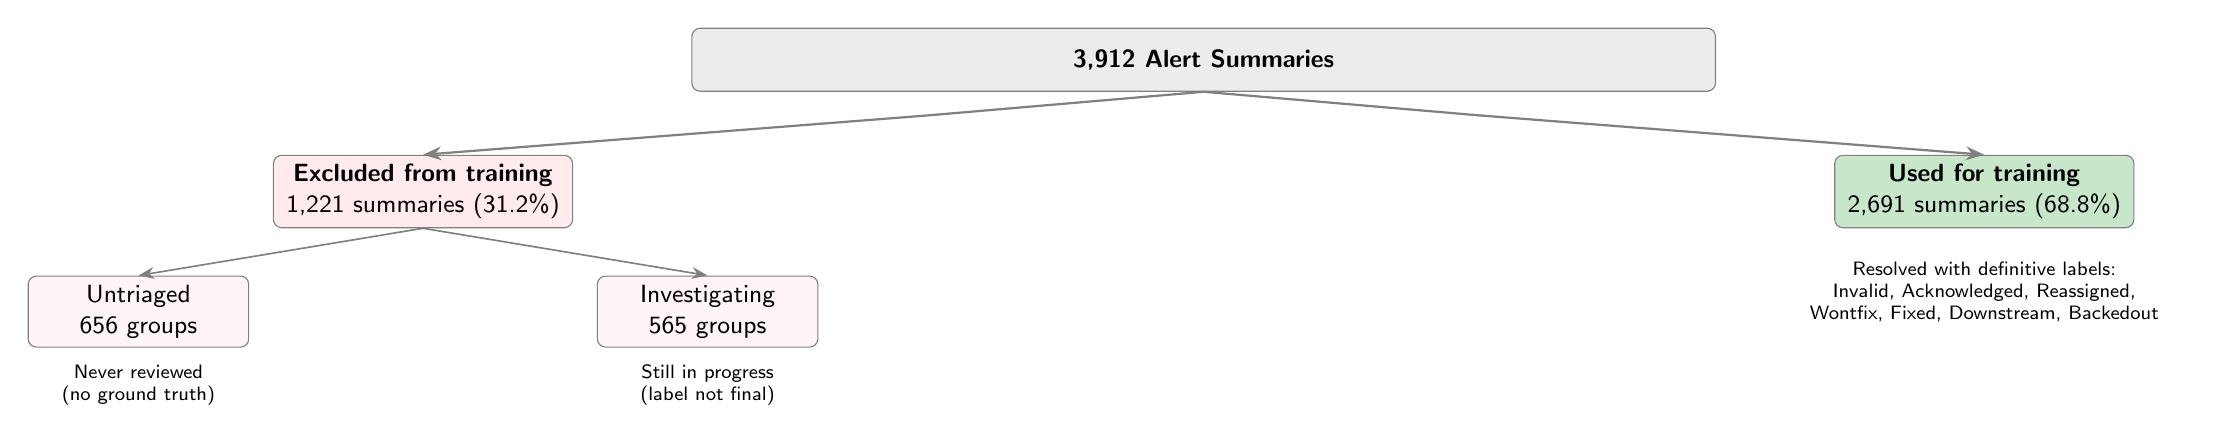
\begin{tikzpicture}[
    node distance=0.3cm,
    box/.style={rectangle, rounded corners=3pt, minimum width=3.8cm,
                minimum height=0.8cm, font=\sffamily\small, draw=gray, align=center},
]

% Total
\node[box, fill=gray!15, minimum width=13cm] (total)
    {\textbf{3,912 Alert Summaries}};

% Split
\node[box, fill=sheriffcolor, below left=0.8cm and 1.5cm of total] (excluded)
    {\textbf{Excluded from training}\\1,221 summaries (31.2\%)};
\node[box, fill=autocolor, below right=0.8cm and 1.5cm of total] (included)
    {\textbf{Used for training}\\2,691 summaries (68.8\%)};

\draw[-{Stealth}, gray, line width=0.8pt] (total.south) -- ++(-3.5cm, -0.3cm) -- (excluded.north);
\draw[-{Stealth}, gray, line width=0.8pt] (total.south) -- ++(3.5cm, -0.3cm) -- (included.north);

% Excluded details
\node[box, fill=sheriffcolor!50, below left=0.6cm and 0.3cm of excluded, minimum width=2.8cm] (untriaged)
    {Untriaged\\656 groups};
\node[box, fill=sheriffcolor!50, below right=0.6cm and 0.3cm of excluded, minimum width=2.8cm] (investigating)
    {Investigating\\565 groups};

\draw[-{Stealth}, gray, line width=0.6pt] (excluded.south) -- (untriaged.north);
\draw[-{Stealth}, gray, line width=0.6pt] (excluded.south) -- (investigating.north);

% Reason
\node[font=\sffamily\scriptsize, text width=2.5cm, align=center, below=0.1cm of untriaged]
    {Never reviewed\\(no ground truth)};
\node[font=\sffamily\scriptsize, text width=2.5cm, align=center, below=0.1cm of investigating]
    {Still in progress\\(label not final)};

% Included details
\node[font=\sffamily\scriptsize, text width=5cm, align=center, below=0.3cm of included]
    {Resolved with definitive labels:\\Invalid, Acknowledged, Reassigned,\\Wontfix, Fixed, Downstream, Backedout};

\end{tikzpicture}%
}% end adjustbox
\caption{Training data selection. Only summaries with definitive, resolved labels are used for training. Investigating and Untriaged summaries are excluded because their labels are uncertain or incomplete.}
\label{fig:training_data}
\end{figure}

\noindent\textbf{Why exclude Investigating?} In the training data, ``Investigating'' is a temporary sheriff state---the sheriff may later change it to Acknowledged, Invalid, or any other label. Training on it would teach the model to mimic human indecision patterns rather than learn to classify resolved outcomes. Instead, the model's own uncertainty naturally produces ``Investigating'' outputs via the confidence gate.

% ============================================================
\section{Estimated Impact}
% ============================================================

Based on the dataset characteristics and expected model performance at each stage:

\begin{figure}[H]
\centering
\adjustbox{max width=\textwidth}{%
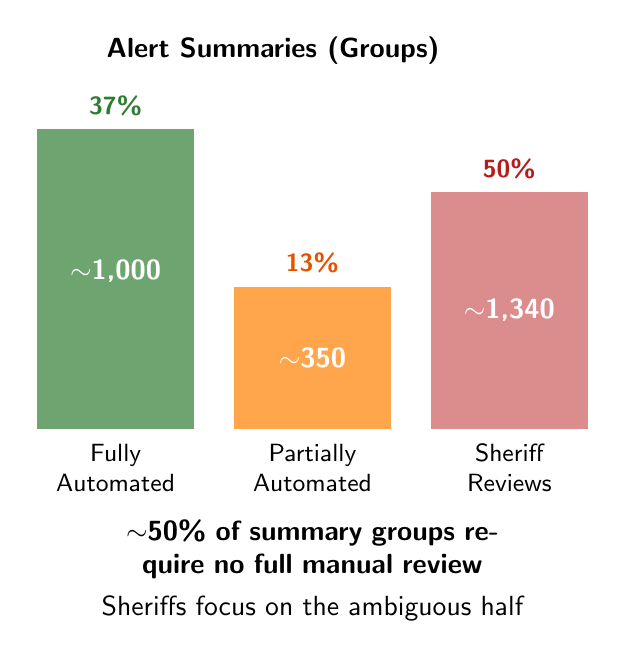
\begin{tikzpicture}
% Bar chart - groups
\begin{scope}[shift={(0,0)}]
\node[font=\sffamily\bfseries, anchor=south] at (3.5, 4.5) {Alert Summaries (Groups)};

% Bars
\fill[darkgreen!70] (0.5,0) rectangle (2.5, 3.8);
\fill[orange!70] (3,0) rectangle (5, 1.8);
\fill[darkred!50] (5.5,0) rectangle (7.5, 3.0);

% Labels
\node[font=\sffamily\small, text width=2cm, align=center] at (1.5, -0.5) {Fully\\Automated};
\node[font=\sffamily\small, text width=2cm, align=center] at (4, -0.5) {Partially\\Automated};
\node[font=\sffamily\small, text width=2cm, align=center] at (6.5, -0.5) {Sheriff\\Reviews};

% Values
\node[font=\sffamily\bfseries, white] at (1.5, 2.0) {$\sim$1,000};
\node[font=\sffamily\bfseries, white] at (4, 0.9) {$\sim$350};
\node[font=\sffamily\bfseries, white] at (6.5, 1.5) {$\sim$1,340};

% Percentages
\node[font=\sffamily\small\bfseries, color=darkgreen] at (1.5, 4.1) {37\%};
\node[font=\sffamily\small\bfseries, color=darkorange] at (4, 2.1) {13\%};
\node[font=\sffamily\small\bfseries, color=darkred] at (6.5, 3.3) {50\%};
\end{scope}

% Arrow and summary
\node[font=\sffamily, text width=6cm, align=center] at (4, -1.8)
    {\textbf{$\sim$50\% of summary groups require no full manual review}\\[3pt]
     Sheriffs focus on the ambiguous half};

\end{tikzpicture}%
}% end adjustbox
\caption{Estimated distribution of 2,691 resolved alert summaries across automation levels. ``Partially automated'' means the group is labeled but some individual alerts need review.}
\label{fig:impact}
\end{figure}

\begin{table}[H]
\centering
\caption{Estimated system performance and workload reduction}
\label{tab:estimates}
\small
\begin{tabular}{lrrr}
\toprule
\textbf{Metric} & \textbf{Current} & \textbf{With System} & \textbf{Savings} \\
\midrule
Groups requiring full manual review & 2,691 & $\sim$1,300 & $\sim$48--55\% \\
Alerts requiring any human review & 11,222 & $\sim$7,200--9,300 & $\sim$17--36\% \\
Groups fully automated & 0 & $\sim$900--1,100 & --- \\
Invalid groups auto-filtered & 0 & $\sim$200--245 & $\sim$41--50\% \\
\midrule
\multicolumn{4}{l}{\textit{Per-stage accuracy on auto-labeled subset}} \\
\midrule
Stage 0 (Invalid filter) & --- & \multicolumn{2}{c}{88--92\%} \\
Stage 1 (Group disposition) & --- & \multicolumn{2}{c}{72--80\%} \\
Stage 2 (Individual alert roles) & --- & \multicolumn{2}{c}{75--82\%} \\
Stage 3 (Bug linkage) & --- & \multicolumn{2}{c}{70--78\%} \\
End-to-end (all stages correct) & --- & \multicolumn{2}{c}{\textbf{65--75\%}} \\
\bottomrule
\end{tabular}
\end{table}

\vspace{0.5em}
\noindent\textbf{Why alert-level savings are lower than group-level:} Invalid groups (which the system catches best) tend to be small (1.75 alerts on average), while the large, complex groups (averaging 8+ alerts) are harder to auto-resolve. The system efficiently handles many small, clear-cut cases while deferring complex multi-alert groups to humans---which is exactly where human judgment adds the most value.

% ============================================================
\section{Safety Properties}
% ============================================================

The cascading confidence-gated design provides several safety guarantees:

\begin{enumerate}[nosep]
    \item \textbf{No silent failures.} Every uncertain prediction is explicitly labeled as code~0 (``Investigating'' / ``not evaluated''). The system never guesses when unsure.

    \item \textbf{Self-correcting cascade.} If Stage~0 incorrectly passes an Invalid group as Valid, Stage~1 will likely be uncertain about it (Invalid groups don't match any disposition class well) and route it to Investigating---where the sheriff catches the error.

    \item \textbf{Conservative errors.} When the system is wrong, errors tend to be low-harm: confusing Acknowledged with Wontfix (both are ``real regression''), or over-deferring to sheriffs (extra human review, but no incorrect auto-labels).

    \item \textbf{Consistent uncertainty encoding.} Code~0 means ``needs human review'' across all three outputs (summary status, alert status, \texttt{has\_bug}), providing a uniform interface for downstream consumers.

    \item \textbf{Human-in-the-loop by design.} The system is designed to \textit{assist} sheriffs, not replace them. It handles the easy 50\% automatically and presents the hard 50\% with partial annotations (noise flags, confidence hints) to accelerate human review.
\end{enumerate}

\end{document}
